\documentclass[journal=jacsat,manuscript=article,layout=twocolumn]{achemso}
%   \usepackage[version=3]{mhchem} % Formula subscripts using \ce{}
\usepackage[T1]{fontenc}       % Use modern font encodings
% \usepackage[active]{preview}
%EXTRA PACKAGES%
% \usepackage{multicol}
\usepackage{xcolor}
\usepackage{textcomp}
\usepackage{geometry}
\usepackage[normalem]{ulem}
\usepackage{amsmath}
\usepackage{amssymb}
% \usepackage{showkeys}
%%%%%%%%%%%%%%%%%%%%%%%%%%%%%%%%%%%%%%%%%%%%%%%%%%%%%%%%%%%%%%%%%%%%%
%% Place any additional macros here.  Please use \newcommand* where
%% possible, and avoid layout-changing macros (which are not used
%% when typesetting).
%%%%%%%%%%%%%%%%%%%%%%%%%%%%%%%%%%%%%%%%%%%%%%%%%%%%%%%%%%%%%%%%%%%%%
\newcommand*{\ga}{\alpha}
\newcommand*{\gb}{\beta}
\newcommand*{\gam}{\gamma}
\newcommand*{\gd}{\delta}
\newcommand*{\eps}{\epsilon}
\newcommand*{\veps}{\varepsilon}
\newcommand*{\gz}{\zeta}
\newcommand*{\gt}{\theta}
\newcommand*{\gi}{\iota}
\newcommand*{\gk}{\kappa}
\newcommand*{\gl}{\lambda}
\newcommand*{\gs}{\sigma}
\newcommand*{\go}{\omega}
\newcommand*{\Gam}{\Gamma}
\newcommand*{\gD}{\Delta}
\newcommand*{\gT}{\Theta}
\newcommand*{\gL}{\Lambda}
\newcommand*{\gS}{\Sigma}
\newcommand*{\gO}{\Omega}
\newcommand*{\pt}[1]{\left( #1\right)}
\newcommand*{\pq}[1]{\left[ #1 \right]}
\newcommand*{\pg}[1]{\left\{ #1\right\}}
\newcommand*{\figref}[1]{\figurename~\ref{#1}}
\newcommand*{\red}[1]{\textcolor{red}{#1}}
\newcommand*{\blue}[1]{\textcolor{blue}{#1}}
\newcommand*{\gray}[1]{\textcolor{gray}{#1}}
% \renewcommand{\baselinestretch}


%%%%%%%%%%%%%%%%%%%%%%%%%%%%%%%%%%%%%%%%%%%%%%%%%%%%%%%%%%%%%%%%%%%%%
%% Meta-data block
%% ---------------
%% Each author should be given as a separate \author command.
%%
%% Corresponding authors should have an e-mail given after the author
%% name as an \email command. Phone and fax numbers can be given
%% using \phone and \fax, respectively; this information is optional.
%%
%% The affiliation of authors is given after the authors; each
%% \affiliation command applies to all preceding authors not already
%% assigned an affiliation.
%%
%% The affiliation takes an option argument for the short name.  This
%% will typically be something like "University of Somewhere".
%%
%% The \altaffiliation macro should be used for new address, etc.
%% On the other hand, \alsoaffiliation is used on a per author basis
%% when authors are associated with multiple institutions.
%%%%%%%%%%%%%%%%%%%%%%%%%%%%%%%%%%%%%%%%%%%%%%%%%%%%%%%%%%%%%%%%%%%%%
\author{Elizaveta Guseva}
\email{elizaveta.guseva@stonybrook.edu}
\affiliation[Stony Brook University]
{Laufer Center for Physical and Quantitative Biology, Stony Brook University, Stony Brook, NY, 
(United States)}
% \altaffiliation{A shared footnote}
% \author{Ronald N Zuckermann}
% \affiliation{Lawrence Berkeley National Laboratory (LBNL), Berkeley, CA (United States)}
% \author{Ken A Dill}
% \email{dill@laufercenter.org}
\phone{+1631 632 5400}
\fax{+1631 632 5405}
\affiliation[Stony Brook University]
{Laufer Center for Physical and Quantitative Biology, Stony Brook University, Stony Brook, NY, 
(United States)}


%%%%%%%%%%%%%%%%%%%%%%%%%%%%%%%%%%%%%%%%%%%%%%%%%%%%%%%%%%%%%%%%%%%%%
%% The document title should be given as usual. Some journals require
%% a running title from the author: this should be supplied as an
%% optional argument to \title.
%%%%%%%%%%%%%%%%%%%%%%%%%%%%%%%%%%%%%%%%%%%%%%%%%%%%%%%%%%%%%%%%%%%%%
\title[]{Resilience and innovability}

%%%%%%%%%%%%%%%%%%%%%%%%%%%%%%%%%%%%%%%%%%%%%%%%%%%%%%%%%%%%%%%%%%%%%
%% Some journals require a list of abbreviations or keywords to be
%% supplied. These should be set up here, and will be printed after
%% the title and author information, if needed.
%%%%%%%%%%%%%%%%%%%%%%%%%%%%%%%%%%%%%%%%%%%%%%%%%%%%%%%%%%%%%%%%%%%%%
\abbreviations{IR,NMR,UV}
\keywords{American Chemical Society, \LaTeX}

%%%%%%%%%%%%%%%%%%%%%%%%%%%%%%%%%%%%%%%%%%%%%%%%%%%%%%%%%%%%%%%%%%%%%
%% The manuscript does not need to include \maketitle, which is
%% executed automatically.
%%%%%%%%%%%%%%%%%%%%%%%%%%%%%%%%%%%%%%%%%%%%%%%%%%%%%%%%%%%%%%%%%%%%%



\begin{document}
 \abstract{Here we will argue that we don't need heredity or adaptive evolution at the early 
stages of life origins, but we need resilience and innovability. We provide a plausible example of 
such chemical system and explain mechanism how such a system can develop in something more. }
 
 
\section{Tests}
\paragraph{Tests to be performed.} 
\begin{enumerate}
 \item [(1)] Genotype variability and resilience over the time (bulk)
 \subitem \textbullet Folders
 \subitem \textbullet Autocats
 \item [(2)] Check presence and diversity of autocats (bulk)
 \item [(3)] Check presence and diversity of the shapes (bulk)
 \item [(4)] Make length comparison studies (bulk)
 \item [(5)] Genotype variability and resilience over the time (vesicles)
 \subitem Folders
 \subitem Autocats
 \item [(6)] Check presence and diversity of autocats (vesicles)
 \item [(7)] Check presence and diversity of the shapes (vesicles)
 \item [(8)] Make length comparison studies (vesicles)
\end{enumerate}
\paragraph{Performed \emph{exploratory} tests.} 
\begin{enumerate}
 \item [(1)] There are few persisting autocats and folders. See integral frequencies distributions 
below.
  \subitem \textbullet\, Folders. Model 18, Simulation 71, Trajectory 0. See figure 
\ref{fig:foldTimeDistr}
  \begin{figure}[htb!]
  \centering
  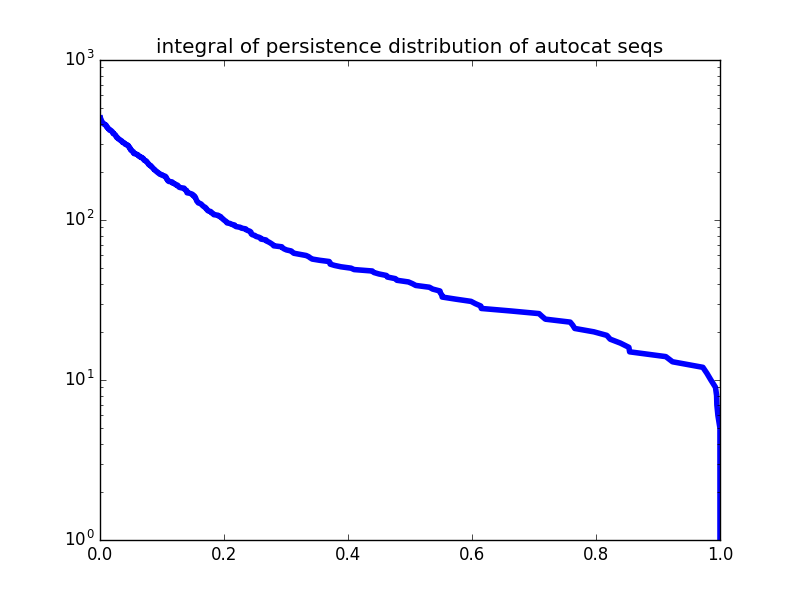
\includegraphics[width=\columnwidth]{inno-fig/exp_foldTimeDistr.png} 
  \caption{Y: how many sequences persist over at least the X part of all time}
  \label{fig:foldTimeDistr}
\end{figure} 
 \subitem \textbullet\, Autocats. Model 18, Simulation 71, Trajectory 0. See figure 
\ref{fig:autoTimeDistr}
 \begin{figure}[htb!]
  \centering
  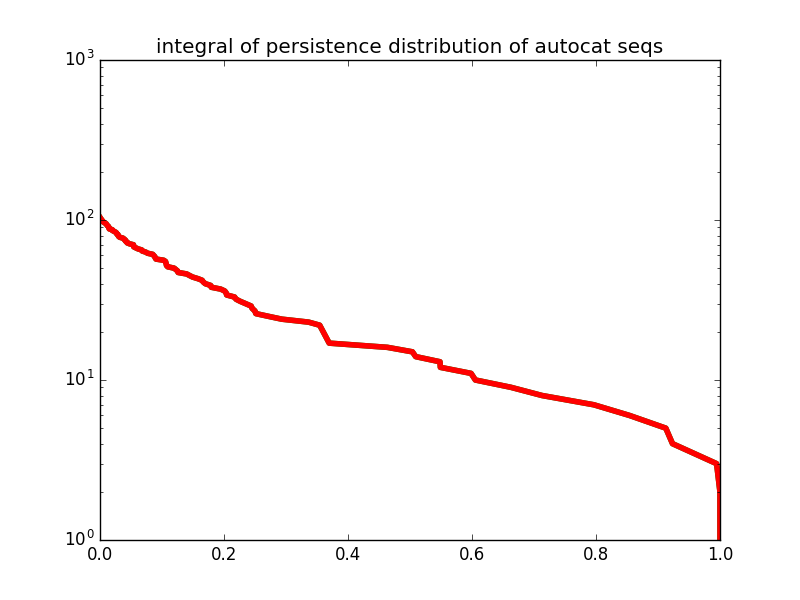
\includegraphics[width=\columnwidth]{inno-fig/exp_autoTimeDistr.png} 
  \caption{Y: how many sequences persist over at least the X part of all time}
  \label{fig:autoTimeDistr}
\end{figure}

 \item [(2)] Testing
 \item [(3)] There are preserved shapes. They are present in very small quantities at import rate 
of 1000. But as the import rates grow, number of shapes grows also.
 \item [(4)] I am not sure if it makes sense
 \item [(5)]
 \item [(6)]Autocats: ['HPPHPHPPPHHHHHHHHHHHHHHH', 'HPHPHPHPHHHHHHHHHHHHH', 
'HPPHPHPHPHHHHHHHHHHHHHHH', 'HPPPHPHHHHHHHHHHHH', 'HPHPHPHPPHHHHHHHHHHH', 'HPHPPPHPPHHHHHHHHHHH']\\
Folders: ['HPPHPHPPPHHHHHHHHHHHHHHH', 'HPHPHPHPHHHHHHHHHHHHH', 'HPHPHPHPPHHHHHHHHHHH', 
'HPHPPPHPPHHHHHHHHHHH', 'HPHPPHPPHPPH', 'HPPPHPHHHHHHHHHHHH', 'HPPHPHPHPHHHHHHHHHHHHHHH']

 \item [(7)]
 \item [(8)]
\end{enumerate}
 
\section{On evolvability of autocatalytic sets }
\subsection{Vasas2012 \citep{Vasas2012}} 
\begin{enumerate}
\item It has been suggested that “...some autocatalytic
sets will reproduce more rapidly than others and
hence will have higher Darwinian fitness” and, therefore,
“we have evolution without a genome"([1], pp. 332-333).
However, no rigorous analysis of the putative evolvability
of autocatalytic sets (but see [4] for a demonstration
of the absence of Darwinian evolution in other models)
has been carried out so far. For example, Bagley and
Farmer [14]
\item Spencerian sense of evolution [15]
\end{enumerate} 
 
\end{document}
